\documentclass{article}[twocolumn]
\usepackage[pdftex]{graphicx}
\usepackage[utf8]{inputenc}
\usepackage[brazil]{babel}
\usepackage{subfigure}
\usepackage{mathtools}
\usepackage{amsmath}
\usepackage{amssymb}
\usepackage{float}
\usepackage{tikz}
\usepackage[a4paper,top=2.5cm,bottom=2.5cm,left=2cm,right=2cm,marginparwidth=1.5cm]{geometry}

\title{Relat\'orio da atividade 4}
\author{Kenji Yamane}

\begin{document}
	\maketitle
	\section{Explora\c{c}\~ao dos dados}
	As seguintes figuras mostram os c\'odigos e figuras geradas para se analisar os dados
	existentes.
	\begin{figure}[H]
		\centering
		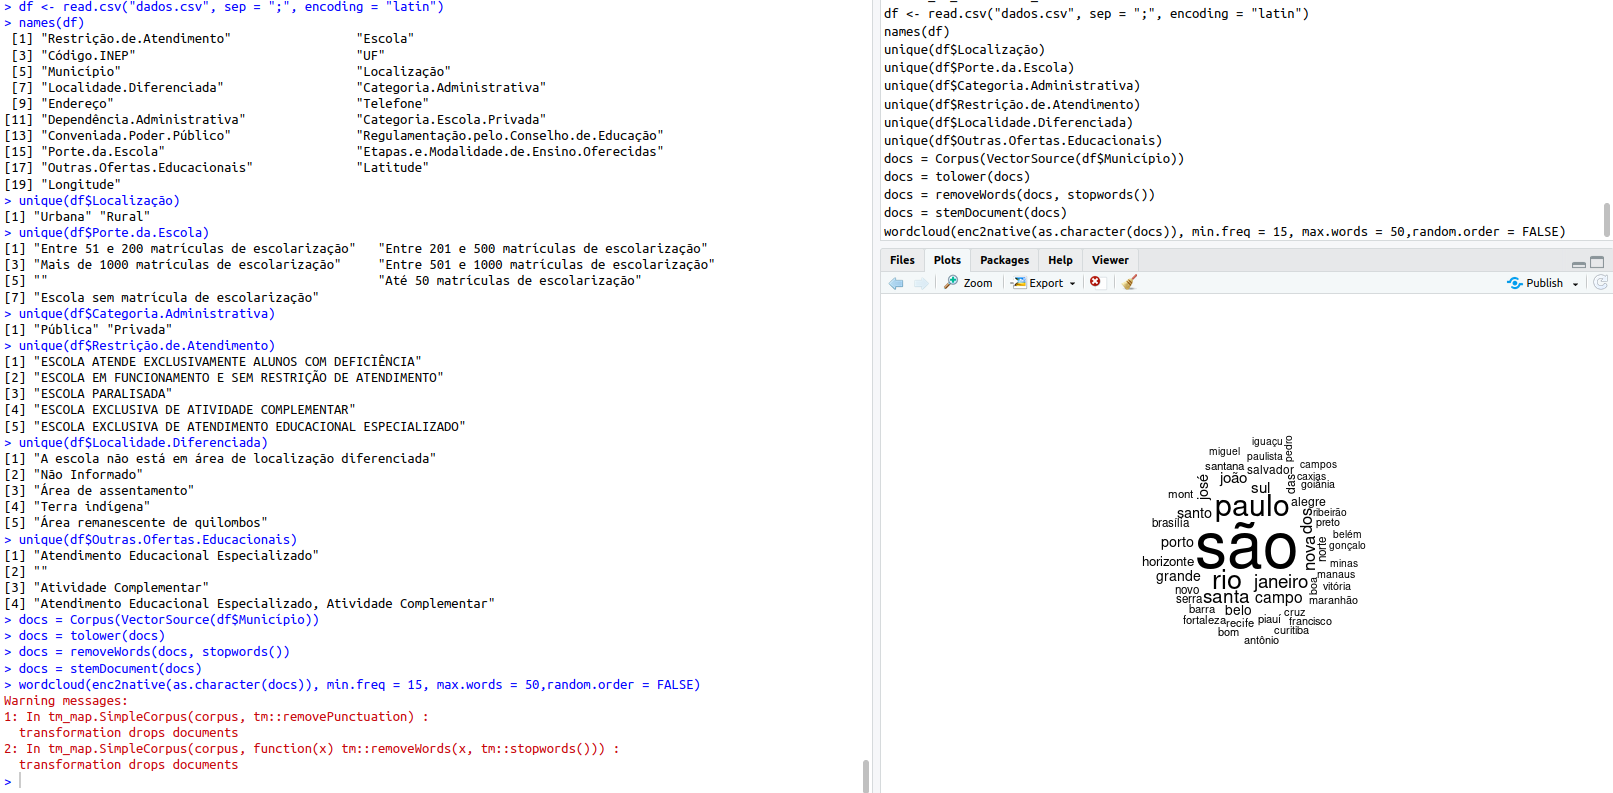
\includegraphics[width=\textwidth]{figures/exploration1.png}
		\caption{Explorando colunas e resumo da coluna \texttt{Municipio}.}
	\end{figure}
	\begin{figure}[H]
		\centering
		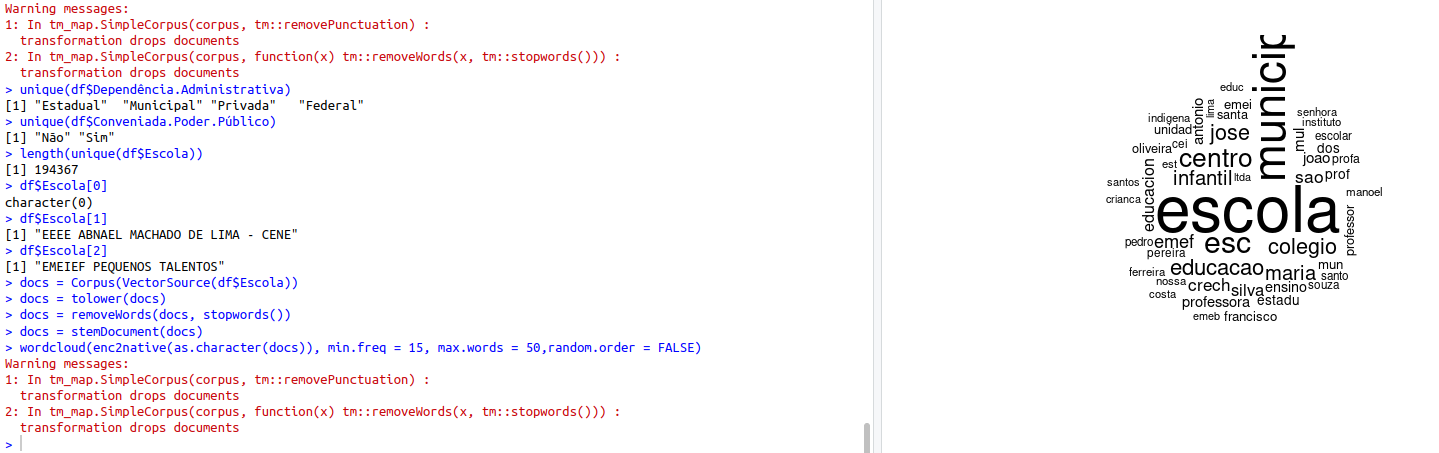
\includegraphics[width=\textwidth]{figures/exploration2.png}
		\caption{Explorando colunas e resumo da coluna \texttt{Escola}.}
	\end{figure}
	\begin{figure}[H]
		\centering
		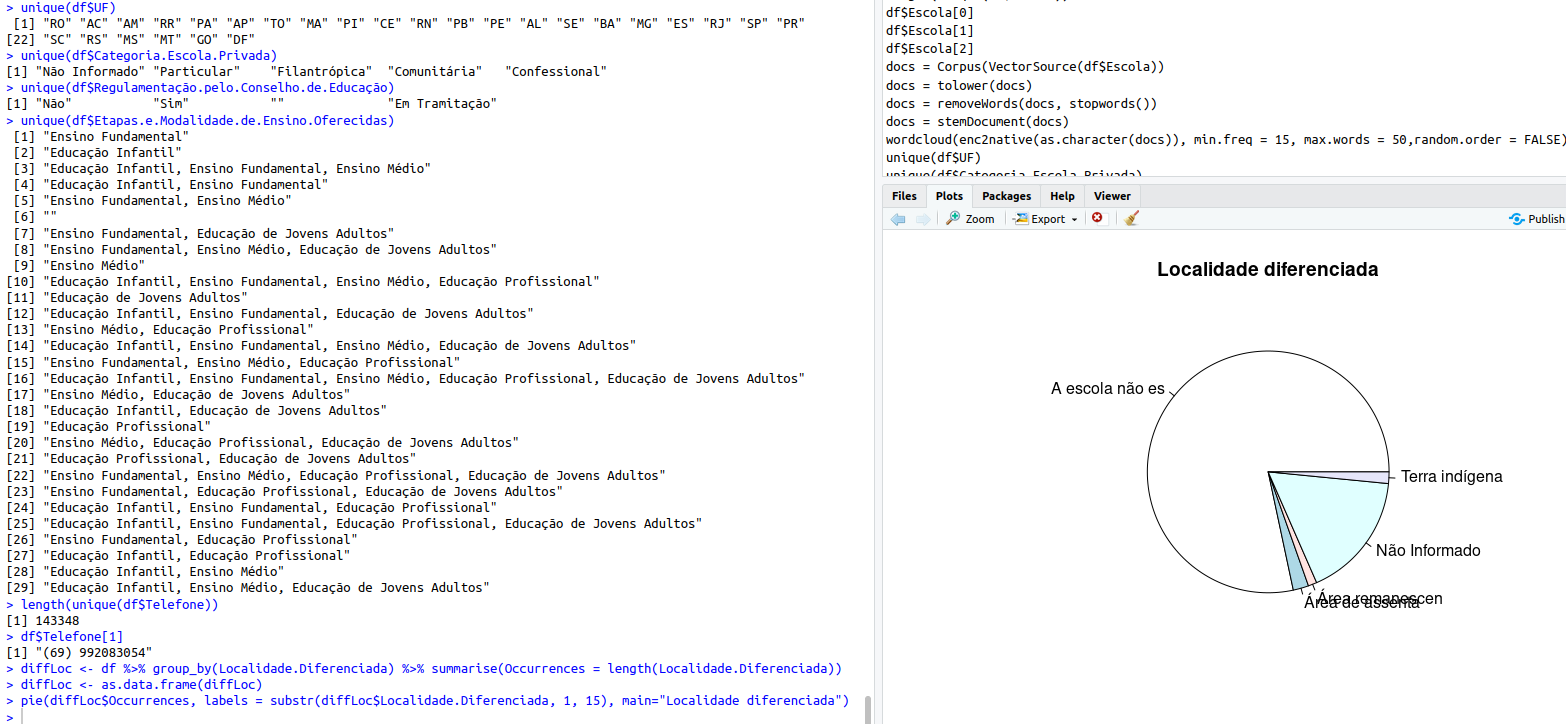
\includegraphics[width=\textwidth]{figures/exploration3.png}
		\caption{Explorando colunas e resumo da coluna \texttt{Localidade diferenciada}.}
	\end{figure}
	\begin{figure}[H]
		\centering
		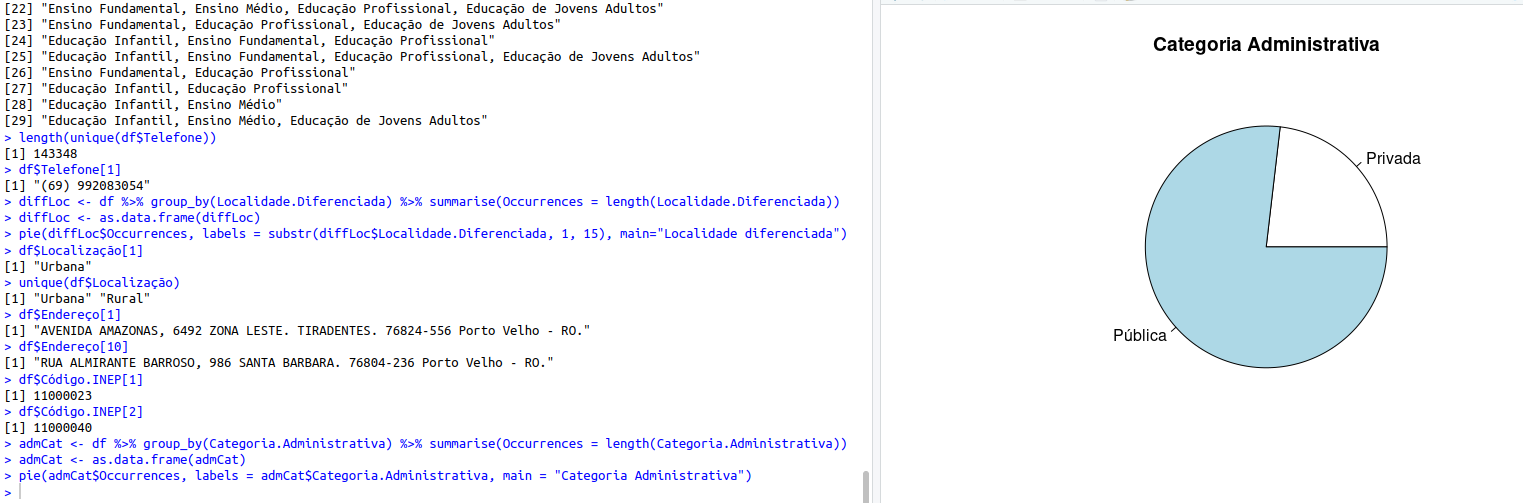
\includegraphics[width=\textwidth]{figures/exploration4.png}
		\caption{Explorando colunas e resumo da coluna \texttt{Categoria administrativa}.}
	\end{figure}
	\section{Manipula\c{c}\~ao de dados}
	Primeiramente, normalizaram-se os dados presentes na coluna \texttt{Etapas e Modalidade de
	Ensino Oferecidas}, quebrando-a em 5 colunas de \texttt{booleanas}, como mostrado na figura
	a seguir:
	\begin{figure}[H]
		\centering
		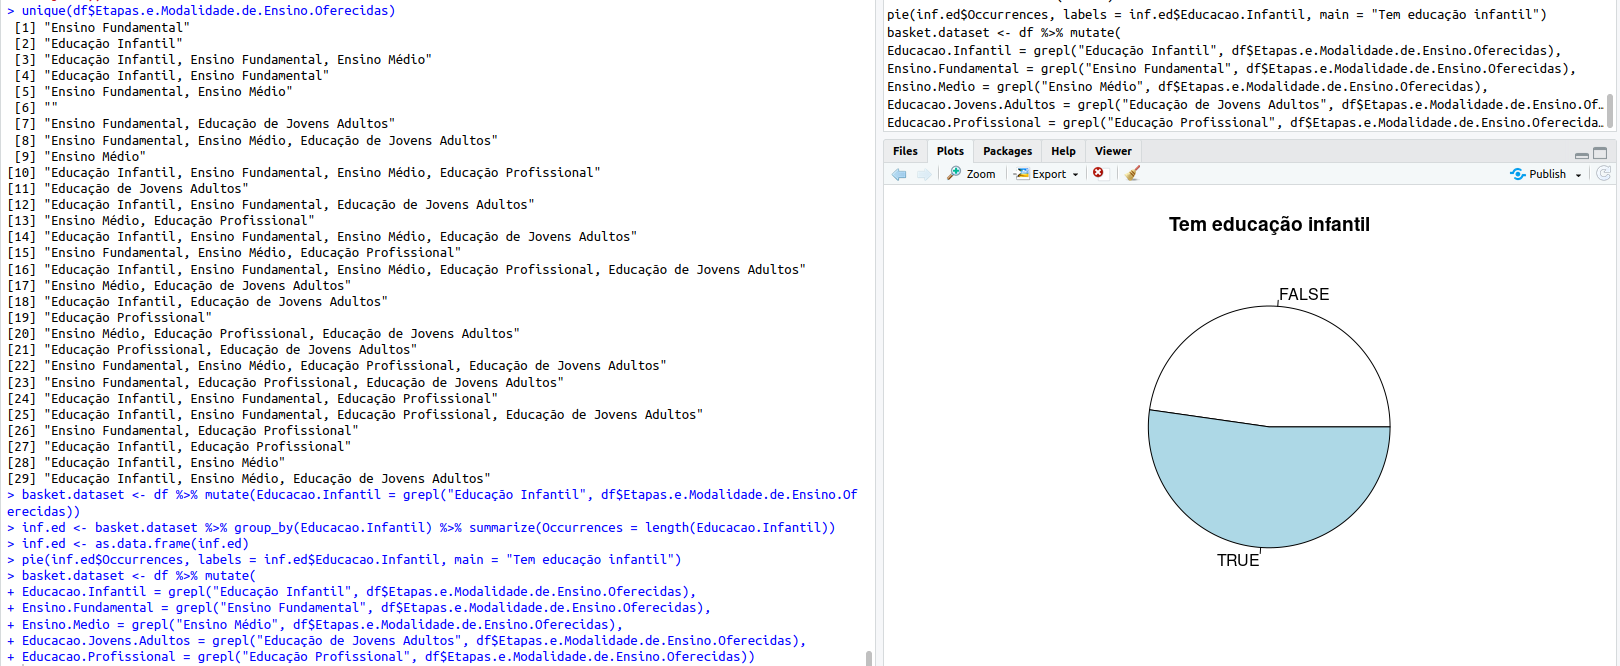
\includegraphics[width=\textwidth]{figures/manipulation1.png}
		\caption{Decomposi\c{c}\~ao da tabela \texttt{Etapas e Modalidade de Ensino Oferecidas}.}
	\end{figure}
	Em seguida, eliminaram-se as colunas n\~ao categ\'oricas:
	\begin{figure}[H]
		\centering
		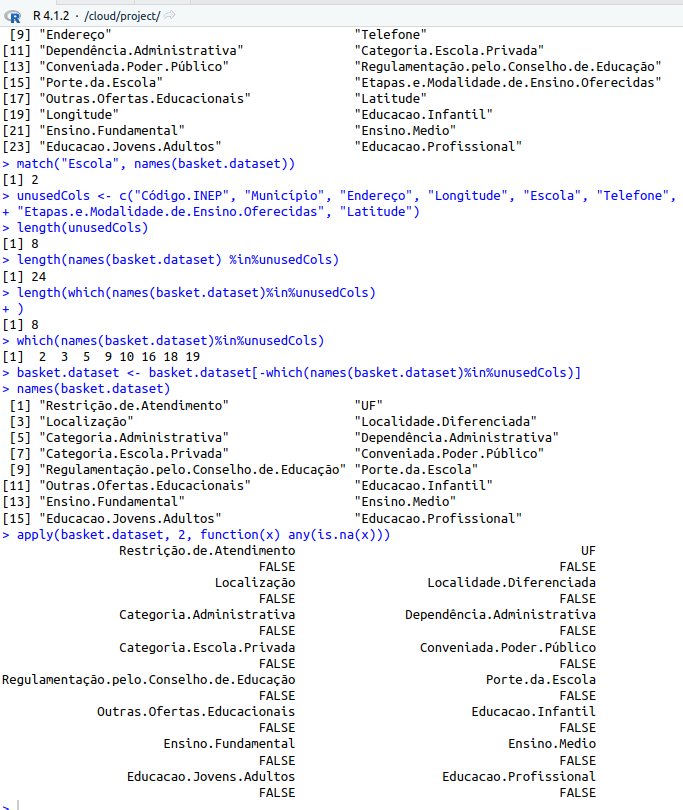
\includegraphics[width=\textwidth]{figures/manipulation2.png}
		\caption{Elimina\c{c}\~ao de colunas n\~ao categ\'oricas.}
	\end{figure}
	\section{An\'alise de dados}
	Eliminando-se algumas colunas para se suportar com a RAM dispon\'ivel de 1 GB,
	procurou-se por regras de associa\c{c}\~ao com \textit{Market Basket Analysis}.
	\begin{figure}[H]
		\centering
		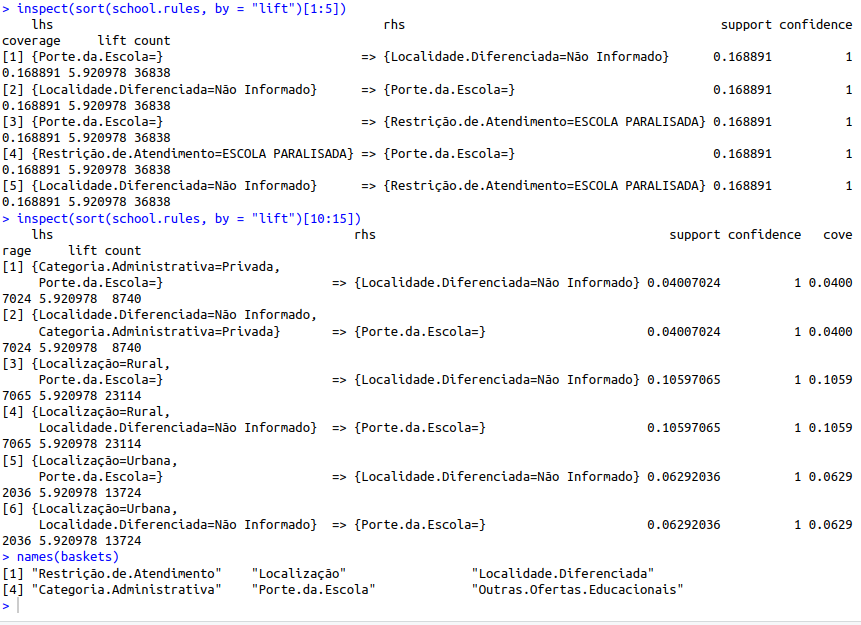
\includegraphics[width=\textwidth]{figures/extraction1.png}
		\caption{Primeira extra\c{c}\~ao de regras de associa\c{c}\~ao.}
	\end{figure}
	Por\'em observa-se uma associa\c{c}\~ao \'obvia entre a aus\^encia de divulga\c{c}\~ao de
	informa\c{c}\~oes.

	Escolhendo-se assim, como transa\c{c}\~oes as seguintes colunas:
	\begin{itemize}
		\item \texttt{Restri\c{c}\~ao de Atendimento}
		\item \texttt{Localidade Diferenciada}
		\item \texttt{Depend\^encia administrativa}
		\item \texttt{Regulamenta\c{c}\~ao pelo Conselho da Educa\c{c}\~ao}
		\item \texttt{Localiza\c{c}\~ao}
		\item \texttt{Categoria Administrativa}
		\item \texttt{Conveniada Poder P\'ublico}
	\end{itemize}
	Obteve-se diversas correla\c{c}\~oes implicadas pela localidade diferenciada:
	\begin{figure}[H]
		\centering
		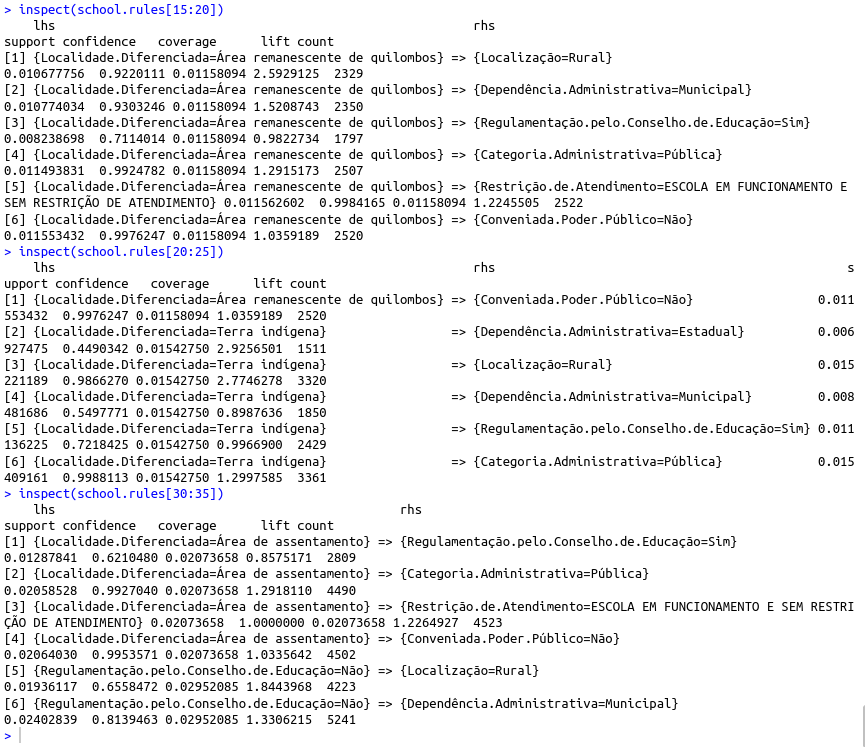
\includegraphics[width=\textwidth]{figures/extraction2.png}
		\caption{Segunda extra\c{c}\~ao de regras de associa\c{c}\~ao.}
	\end{figure}
\end{document}
